\documentclass[conference]{IEEEtran}
%
% *** GRAPHICS RELATED PACKAGES ***
%
%\usepackage[pdftex]{graphicx}
\usepackage{graphicx}
\usepackage{subfig}
\usepackage{listings}
\usepackage{enumitem}
\usepackage{hyperref}
\usepackage{todonotes}

%
% Local Macros
%
\newcommand{\term}[1]{\emph{#1}}

%\usepackage{subcaption}
% declare the path(s) where your graphic files are
\graphicspath{{../figures/}}
% and their extensions so you won't have to specify these with
% every instance of \includegraphics
\DeclareGraphicsExtensions{.pdf,.jpeg,.png,.jpg,.eps}

% correct bad hyphenation here
\hyphenation{op-tical net-works semi-conduc-tor}

\begin{document}
%
% Linebreaks \\ can be used within to get better formatting as desired.
%
\title{What is a Polystore?}
%
% author names and affiliations
% use a multiple column layout for up to three different affiliations
%
\author{\IEEEauthorblockN{
           Timothy G Mattson\IEEEauthorrefmark{1} 
           Michael Stonebraker\IEEEauthorrefmark{2}
           David Maier\IEEEauthorrefmark{3}
           Bill Howe\IEEEauthorrefmark{4}
           Dylan Hutchison\IEEEauthorrefmark{4}
           Shrainik Jain\IEEEauthorrefmark{4}}
        \IEEEauthorblockA{
           \IEEEauthorrefmark{1}Intel Corp.
           \IEEEauthorrefmark{2}MIT CSAIL 
           \IEEEauthorrefmark{3}Portland State University
           \IEEEauthorrefmark{4}University of Washington}
}

% make the title area
\maketitle

\let\thefootnote\relax\footnotetext{The corresponding author, Tim Mattson, 
can be reached at timothy.g.mattson [at] intel.com}

\begin{abstract}

Big Data problems often result in heterogeneous
data distributed across multiple databases.  
In response a wide range of systems have been created
with labels such as
{\emph data federation}, 
{\emph multistores}, {\emph polystores}, and more.  In 
the literature these system overlap in confusing ways making it quite 
difficult to understand how these systems compare.

In this paper, we propose a set of definitions for these
multiple-datastore systems resulting in a precise definitions
for the terms {\emph multistore} and {\emph polystore}.  
We then survey the literature and assign 
different systems to our framework of definitions.
Finally, we provide a set of rules to help constrain what is and
is not a Polystore system.

\end{abstract}

% no keywords

\IEEEpeerreviewmaketitle

\section{Introduction}

Many applications are built around heterogeneous 
data organized into multiple databases.  This trend will most
assuredly grow over time.   Furthermore, there is great value
both in terms of the ease of constructing queries and in the 
efficiency of execution, to matching data to the 
storage engine.  This is captured by the now famous
slogan that ``one size does not fit all'',~\cite{Stonebraker2005one}

We proposed the term 
\term{polystore}~\cite{Duggan2015,Elmore2015demo,Gadepally2016}
to describe our work on database management systems for 
complex heterogeneous data.  As we have shown 
elsewhere~\cite{Elmore2015demo} that we can use the
polystore concept to build a DBMS system where exploiting the 
heterogeneity in the data stores resulted in improved performance.  
We leave, for example, waveform data in an array storage engine and 
relational data in a a relational storage engine. Queries spanning the 
two systems, even when extra copy overhead is included, are 
faster than forcing the data into a single system.

Given the growing complexity of data sets, we expect (and hope) 
systems utilizing the features of multiple data stores will
become a major research thrust across the academic community.
Before this happens and multiple data store terminology becomes 
part of the jargon of computer science, however, we want to 
firmly establish a useful set of definitions.   
There is a long history of computer scientists 
adopting terms and modifying them over time
until they loose any precise definition.  Eventually, 
the terms loose any connection to the original concept.  A classic 
example is the word \term{paradigm} originally from Thomas Kuhn's 
classic work on the structure of scientific revolution~\cite{Kuhn1962}  
and now used by computer scientists to reference any new 
approach to one's favorite computer science problem.

We want to prevent this fate from befalling terms such as
\term{polystore} and \term{multistore} and help them
retain useful, precise meanings as others adopt these terms 
in their own research.  That is the primary purpose of this paper.   
Along the way, we hope to bring clarity to other terms commonly used 
(and misused) in the database community.

We will accomplish this task in two ways.  First, inspired by Guy Steele's 
OOPSLA talk in 1998~\cite{Steele98}, we will develop our definition
of \term{polystore} step by step starting with basic definitions 
from the database research community and working our way up 
to the \term{polystore}.  This may seem cumbersome, but given the 
confused state of terminology in computer science, this is the only way 
to make sure the context as well as the definition of polystore is 
clear.  Next, we will follow the example of Codd with his 
famous 12~rules ~\cite{Codd85} that any system calling itself a 
relational database must satisfy; defining our own rules any 
polystore system must satisfy.

We then describe our own polystore prototype system, 
BigDAWG~\cite{Duggan2015} and how it relates to our polystore
rules.  We close with a discussion of related database systems 
relative to our rules to understand other approaches to the Polystore concept. 

%in Section~\ref{Polystore} 

\section{Database Definitions Framework}
\label{DefFramework}

We begin with core definitions applicable across all modern
database management systems. This first set of definitions
pertains to the persistent storage of data.

\begin{itemize}

\item \term{Data Store}: A system that 
provides persistent storage for data and access methods to 
store and/or retrieve that data.   

\item \term{Data Model}: Abstractions that define the 
structures around which data is organized, constraints on values
of the data, and a set of operators
over those structures. An example of a data model would be 
a relational algebra.

\item \term{Storage Engine}: A Data Store supporting the data 
structures from a  particular data model.  Access methods support
low level IO operations but not complex queries.  
Examples: InnoDB, H-Store, TileDB, HDFS.
\end{itemize}

Users explore data posting requests 
to find specific facts or complex relationships 
between data elements.  

\begin{itemize}

\item \term{Query}: A request that can be translated into an 
expression composed of operators from a data model.  
A \term{Query language} is a language or API used to 
construct queries.

\item \term{Query Plan}: The physical 
implementation of a Query.

\item \term{Query Engine}: a software component that
executes a query plan based on the operators in a data model. 
Typically, a Query engine is tightly coupled to an associated
storage engine.  Example of a stand-alone query engine 
is Datomic (http://blog.datomic.com/).  

\item A \term{Database} is a collection of data organized according
to a high level data model and accessed through operators 
defined in that model.

\item A \term{Database Management System} or \term{DBMS} 
utilizes one or more storage engines and one or more query engines 
to implement the functionality required to manage a database.  This
includes data definition, update, retrieval, and administration 
(monitoring, security, resilience, integrity, and concurrency control).  

\end{itemize}

The concept of presenting multiple databases as a single
system~\cite{Nordbotten1991} is well established.  

\begin{itemize}
\item \term{Data Warehouse} A DBMS holding data injessted from
multiple databases.  If the data is unstructured is it called
a \term{data lake}.
 
\end{itemize}

The more interesting case for our purposes, hjowever, is cases
where data remains in the storage engine suited to the data.   
This leads to systems composed of multiple DBMS.


\item \term{Multi-DBMS}: a data management system composed of 
multiple DBMS systems.  Queries to the system are expressed
in terms of an application programming interface supported 
by a single top-level query engine.

\end{itemize}

Different Multi-DBMS systems are characterized 
by the degree of integration between the database management systems.
At one extreme are cases where the database management systems are
autonomous (i.e. not integrated).

\begin{itemize}
\item \term{federated DBMS}: A Multi-DBMS system composed of multiple 
independently managed, autonomous DBMSs.   Any integration 
between DBMS systems is virtualized through the data federation query
engine.

\end{itemize}

When the systems are integrated and managed as a single system,
we distinguish between systems based on whether the storage engines
are homogeneous or heterogeneous.  

\begin{itemize}

\item \term{Multi-store}: A DBMS system composed of multiple storage 
engines.  The multistore system has a top-level query engine and associated
API which makes the multistore system appear as a single DMBS.
A single query using the multistore's API may resolve into operators 
over multiple storage engines, but those engines may use a common data model. 

\item \term{Poly-store}: A multi-store system that accepts
queries that resolve into operators executing over storage engines that 
support multiple, different data models.  
The storage engines are fully exposed so (1) placement decisions are 
explicit in a polystore system and (2) the full capability of the
individual storage engines are fully exposed.

\end{itemize}

distributed database management system.  Implements a storage
engine that has been parallelized.  It's a single storage engine
that has been decomposed to run on multiple machines.  Hence, 


Another common multi-DBMS use case occurs when data is partitioned
into smaller units that are run on a distributed system within
replicated instances of a single DBMS.  For example, in a large
relational database, the partitions are horizontal meaning 
rows of the table are partioned and mapped to different
nodes in a distributed system.  These are well 
distributed data bases.  

These definitions result in a hierarchical organization of 
systems as shown in figure~\ref{fig:defs}.

\begin{figure*}[t!]
\centerline{
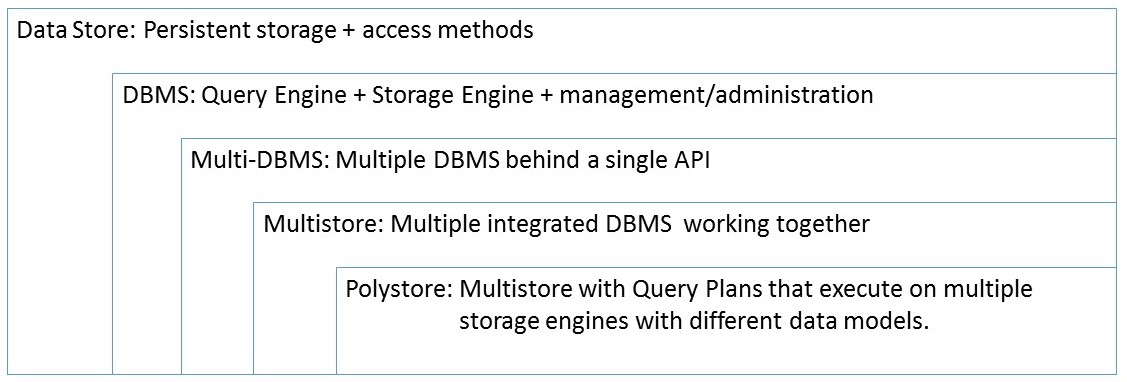
\includegraphics[width=7.0in]{figures/systems.jpg}
}
\caption{A visual representation of the relations between
  definitions leading up to polystore.}
\label{fig:defs}
\end{figure*}

SQL server is a multistore but not a polystore.  It has three query
engines, the row-store, the column-store, and a in-memory 
engine (hecaton).   These are three query engines each managing
their storage but they are all based on a single data model.  And you 
have to choose where the data goes between the three.


In designing a Polystore system, the challenge is to balance the
two competing forces:
\begin{itemize}

\item \term{Store Transparency}: the property of a query in a 
polystore system to move transparently between data stores. This 
is a great convenience for programmers.

\item \term{Semantic completeness}: The ability in a polystore system
to fully exploit any of the component storage engines in the system.

\end{itemize}

Store Transparency lets a data user issue queries without having
to understand which storage engines are used in the query.  This 
creates a separation of concerns between the data user and the
database designer giving the database designer flexibility to map
data between storage engines to optimize performance.   Almost
by design, however, store transparency reduces the ability to
design queries around the features of a specific engine; i.e. 
store transparency abstracts the query away from the specific
features of a storage engine and compromises the ability to exploit
the full set of features in a storage engine.   Later we will
see how we balance these two forces in our prototype 
polystore system, BigDAWG.

\section{Rules}

%
%  We might also explicitly call out non-requirements (though 
% I don't have any in mind at the moment -- perhaps that we don't 
% mandate a specific internal architecture, or that every polystore 
% deployment have exactly the same stores -- Bill has run across 
% some cases where different users might even seen different 
% capabilities). Perhaps update is a non-requirement: if we are 
% in the data analytics area, then datasets might be immutable.
%

A system must satisfy all of the following rules in order
to be called a \term{Polystore system}.
\begin{itemize}

\item {\bf Rule 0}: 
A polystore system must contain multiple storage engines 
at least two of which utilize a different data model.
\begin{quote}
For example, a polystore system might have two relational
and one key-value storage engines.
\end{quote}

\item {\bf Rule 1}: 
All storage engines must be accessible through a single API. 

\item {\bf Rule 2}: 
Data users must be able to construct queries that target the 
specific features of a particular storage engine.

\item {\bf Rule 3}: 
The system must support queries that utilize multiple storage engines 
hence there must be some mechanism to move data directly between 
storage engines. 

\end{itemize}

\section{BigDAWG}

In this section I'll very briefly describe BigDAWG and how it meets
the definition of a polystore. I'll then go over our rules and how
BigDAWG satisfies the rules.

\section{Other systems}

We'll present a table with rows based on the set of definitions
and populate the table with systems.  The text will amplify some of
our decisions concerning where different systems are placed.

Basically, if a single data model is used to expose multiple 
storage engines, I'm calling the sytsem a multistore.  If 
the query engine that exposes the storage engine supports multiple
data models, I'm calling it a polystore.  

I put Myria under the multistore category to see if our freinds
in Seattle are paying attention, but also because it appears to 
me as a casual user of Myria that its strength is the single data model
based on an extended SQL exposes all the storage engines.  But I'm 
eager to be told why I'm wrong.

\begin{table}[h!]
  \centering
  \caption{Systems alligned to our definition framework.}
  \label{tab:relWrk}
  \begin{tabular}{l|l}
    \hline
    Data Federation  & Garlic~\cite{Carey1995towards} \\
                     & IBM DB2~\cite{Gassner1993query}\\
    \hline
    Multistore       & Myria~\cite{Halperin2014demo} \\
                     & MISO~\cite{miso2014}  \\
                     & Odyssey~\cite{odyssey2013}\\
                     & Polybase~\cite{polybase2013}\\
    \hline
    Polystore        & BigDAWG~\cite{Duggan2015,Gadepally2016} \\
                     & CloudMdSQL~\cite{cloudMdSQL2016} \\
                     & Musketeer~\cite{musketeer2015}\\
  \end{tabular}
\end{table}

\section{Conclusion and Discussion}
\label{conc}

Polystore systems are really great.  Everyone should build them
and use them as much as possible.

We need to be forthright that polystores are a developing area, 
and we don't know yet what will be realizable. So perhaps there 
are some base requirements (such as multiple storage engines, 
single queries can use multiple engines, single API), plus desirable 
properties (store transparency, semantic completeness, direct 
interconnect of storage engines, language integration). Right now, 
we don't know whether we can simultaneously satisfy all the desirable 
properties. We have different approaches that are emphasizing one 
and seeing how far they can go towards the other. BigDAWG starts 
from semantic completeness, Myria starts from transparency.

\section*{Acknowledgement}
This work was supported in part by the Intel Science and Technology
Center (ISTC) for Big Data (\url{http://mimic.physionet.org/}).


\bibliographystyle{IEEEtran}
\bibliography{bigdawg.bib}

% that's all folks
\end{document}


